\section{Linear Independence}
\label{sec:linear-independence}

A collection of vectors is useful as a coordinate framework only when none of its members is redundant.

\subsection{Definition}

Vectors $\mathbf v_1,\ldots,\mathbf v_n$ are linearly independent if
\[
c_1\mathbf v_1+\cdots+c_n\mathbf v_n=\mathbf 0
\]
implies
\[
c_1=\cdots=c_n=0.
\]
If a nontrivial choice of coefficients produces the zero vector, the vectors are linearly dependent.

\begin{physical}
Linear dependence means that at least one proposed direction can be reconstructed from the others. It therefore contributes no new degree of freedom.
\end{physical}

\begin{bookfigure}{Independent vectors contribute genuinely different directions; dependent vectors repeat information already present.}
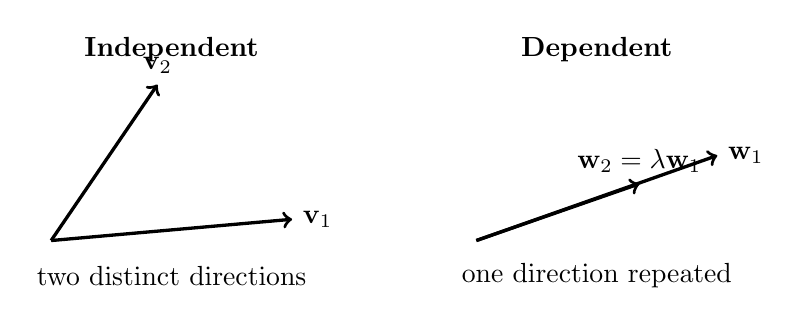
\begin{tikzpicture}[scale=0.9]
  \node[font=\bfseries] at (2.0,3.2) {Independent};
  \draw[->,very thick] (0.3,0.5)--(3.7,0.8) node[right] {$\mathbf v_1$};
  \draw[->,very thick] (0.3,0.5)--(1.8,2.7) node[above] {$\mathbf v_2$};
  \node at (2.0,0.0) {two distinct directions};
  \begin{scope}[xshift=6cm]
  \node[font=\bfseries] at (2.0,3.2) {Dependent};
  \draw[->,very thick] (0.3,0.5)--(3.7,1.7) node[right] {$\mathbf w_1$};
  \draw[->,very thick] (0.3,0.5)--(2.6,1.3) node[above] {$\mathbf w_2=\lambda\mathbf w_1$};
  \node at (2.0,0.0) {one direction repeated};
  \end{scope}
\end{tikzpicture}

\end{bookfigure}

\begin{bookfigure}{Two nonparallel vectors span a plane: every vector in it has the form $a\mathbf v_1+b\mathbf v_2$.}
\begin{tikzpicture}[x=1cm,y=1cm]
\fill[softblue] (-.4,.2)--(4.6,-.25)--(6.0,2.7)--(1,3.2)--cycle;
\draw[book locus] (-.4,.2)--(4.6,-.25)--(6.0,2.7)--(1,3.2)--cycle;
\coordinate (O) at (1.1,.7);
\draw[book vector] (O)--(4.3,.45) node[right] {$\mathbf v_1$};
\draw[book vector secondary] (O)--(2.35,2.55) node[above] {$\mathbf v_2$};
\draw[book accent,-{Latex[length=2mm]}] (O)--(4.75,2.15) node[above right] {$a\mathbf v_1+b\mathbf v_2$};
\node at (3.25,3.25) {$\operatorname{span}\{\mathbf v_1,\mathbf v_2\}$};
\end{tikzpicture}

\label{fig:span-plane}
\end{bookfigure}

\subsection{Geometric Interpretation}

In two dimensions, two nonzero vectors are independent precisely when they are not parallel. In three dimensions, three vectors are independent precisely when they are not coplanar. For three vectors $\mathbf a,\mathbf b,\mathbf c$, the scalar triple product provides a test:
\[
\mathbf a\cdot(\mathbf b\times\mathbf c)\neq0.
\]
Its absolute value is the volume of the parallelepiped spanned by the vectors.

\begin{workedexample}
The vectors $(1,0,1)$, $(0,1,1)$, and $(1,1,2)$ are dependent because
\[
(1,1,2)=(1,0,1)+(0,1,1).
\]
The third vector adds no new direction.
\end{workedexample}

\begin{propertybox}[Matrix test]
Place the candidate vectors as columns of a matrix $M$. For a square set, the vectors are linearly independent exactly when $\det M\neq0$. More generally, independence means that the rank of $M$ equals the number of columns.
\end{propertybox}
